\begin{frame}[allowframebreaks]
	\frametitle{Introduction}
	\par Spiking Neural Networks (SNNs) mimic the workings of the brain by utilizing action potentials, in contrast to continuous values transmitted between neurons.
	
	\par The term "Spiking" originates from the behavior of biological neurons, which sporadically emit action potentials, creating voltage spikes that convey information \cite{kasabov2019time}. Figure \ref{fig:neuronspikes} illustrates these spikes.
	
	\par An SNN \textbf{is not} a one-to-one simulation of neurons. Instead, it approximates certain computational capabilities of specific biological properties. Some studies explore the nonlinearity of dendrites and other neuron features \cite{jones2020single}, yielding remarkable results in the classification.
	
	\begin{figure}[H]
		\centering
		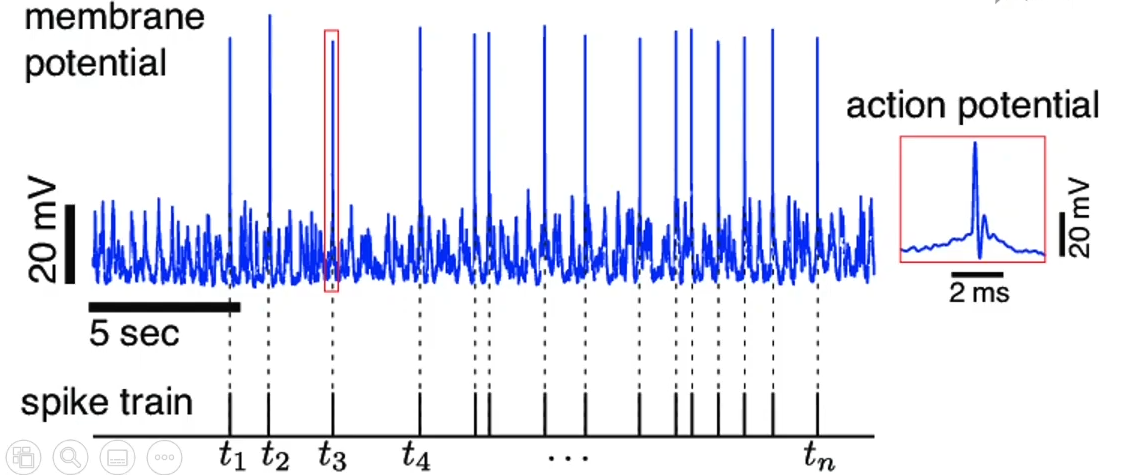
\includegraphics[width=\linewidth]{images/neuronSpikes}
		\caption{Spikes from a noisy signal. Source \cite{dan_goodman_2022_7044500}}
		\label{fig:neuronspikes}
	\end{figure}
\end{frame}

\begin{frame}
	\frametitle{General characteristics}
	
	\par SNNs possess several noteworthy characteristics that distinguish them from traditional machine learning techniques, including classical neural networks. These distinctions encompass \cite{kasabov2019time}:
	
	\begin{itemize}
		\item Proficiency in modeling temporal, spatial-temporal, or spectro-temporal data.
		\item Effectiveness in capturing processes involving various time scales.
		\item Seamless integration of multiple modalities, such as sound and vision, into a unified system.
		\item Aptitude for predictive modeling and event prediction.
		\item Swift and highly parallel information processing capabilities.
		\item Streamlined information processing.
		\item Scalability, accommodating structures ranging from a few tens to billions of spiking neurons.
		\item Minimal energy consumption when implemented on neuromorphic platforms.
	\end{itemize}

\end{frame}

\begin{frame}[allowframebreaks]
	\frametitle{Energy characteristics}
	
		\par Spiking Neural Networks (SNNs) are often considered power-efficient for several reasons:
		
		\par \textbf{Event-Driven Processing}: SNNs are inherently event-driven. Instead of constantly updating neuron activations and synapse weights as in traditional artificial neural networks (ANNs), SNNs only transmit spikes (action potentials) when a neuron's membrane potential reaches a certain threshold. This event-driven approach reduces the amount of computation required and can lead to significant energy savings.
		
		\par \textbf{Sparse Activity}: SNNs tend to exhibit sparse activity, meaning that only a small percentage of neurons are active at any given time. This sparsity reduces the number of computations that need to be performed, which is especially beneficial for hardware implementations where most of the energy consumption comes from active components.
		
		\par \textbf{Low Precision}: SNNs can often work with lower precision than ANNs. While ANNs typically use high-precision floating-point numbers for neuron activations and synaptic weights, SNNs can use lower precision fixed-point or binary representations. Lower precision computations require less energy to perform.
		
		\par \textbf{Neuromorphic Hardware}: SNNs can be efficiently implemented on specialized neuromorphic hardware, which is designed to mimic the energy-efficient behavior of biological neural systems. These hardware platforms are optimized for the event-driven nature of SNNs, further reducing power consumption.
		
		\par \textbf{Energy-Aware Learning Rules}: SNNs can employ learning rules that take into account energy efficiency. For example, some learning rules prioritize strengthening or weakening synapses based on their contribution to network activity, which can lead to more energy-efficient learning.
		
		\par \textbf{Spike Encoding}: SNNs can encode information in the timing and frequency of spikes, which can be a highly efficient way to represent and process data, particularly for event-based sensors like vision sensors or auditory sensors.
\end{frame}

\begin{frame}
	\frametitle{Theory: Spikes and potencials}
	
	\begin{columns}
		\column{0.5\textwidth}
			\par In order to emulate such behavior, let's begin with a simple model: The "Leaky Integrate and Fire neuron" (LIF). The LIF model describes the evolution of membrane potential which the potential decay over time.
			\begin{equation}
				\tau \cdot \frac{dV}{dt} = -V
				\label{eq:leak}
			\end{equation}
			
			\par When a neuron receives a spike, the membrane potential $V$ increases according to a synaptic weight $w$.
			\begin{equation}
				V = V + w
			\end{equation}
			
			\par Such behaviors are depicted in Figure \ref{fig:neuronspikes2}.
		\column{0.5\textwidth}
			\begin{figure}
				\centering
				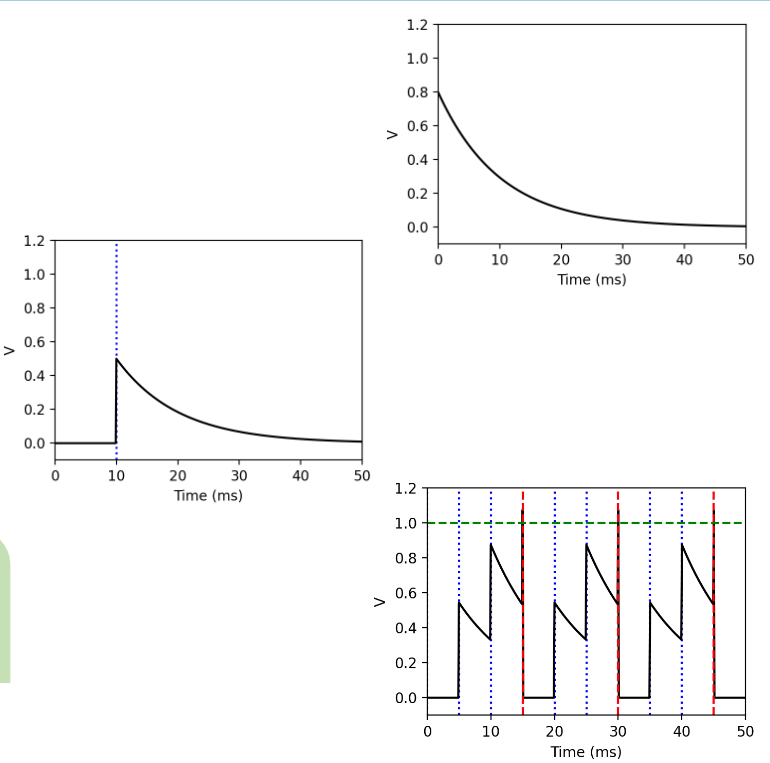
\includegraphics[width=.87\linewidth]{images/neuronSpikes2}
				\caption{Evolution of a Spike. Source \cite{dan_goodman_2022_7044500}}
				\label{fig:neuronspikes2}
			\end{figure}
	\end{columns}

\end{frame}

\begin{frame}
	\frametitle{Theory: Training}
	\par As shown in Figure \ref{fig:neuronspikes2}, when a neuron reaches a certain threshold, it resets ($V = 0$). Note that $V=0$ is just one of the possible values of reset, after this the neuron may or may not enter in a refractory period. \textbf{These, an another values cited ahead, can be parameterized or learned}.\newline
	
	\par \textbf{How do SNNs get trained?} Well, this is still an open question. An SNN neuron has an activation-function behavior that is more relatable to a \textbf{step function}. Therefore, in principle, we can't use gradient descent-based solutions because this kind of function \textbf{is not} differentiable \cite{kasabov2019time}.\newline
	
	\par But there are some insights out there that may shed some light on this subject: While some \textit{in vivo/in vitro} observations show that brains, in general, learn by strengthening/weakening and adding/removing synapses or even by creating new neurons or other cumbersome methods like RNA packets, there are some more acceptable ones like the ones in the slide \cite{kasabov2019time}:

\end{frame}

\begin{frame}
	\frametitle{Theory: Training}
	\begin{itemize}
		\item Spike Timing-Dependent Plasticity (STDP): The idea is that if a pre-synaptic neuron fires \textbf{before} the post-synaptic one, there is a strengthening in connection, but if the post-synaptic neuron fires before, then there is a weakening.
		\item Surrogate Gradient Descent: The technique \textbf{approximates} the step function by using another mathematical function, which is differentiable (like a sigmoid), in order to train the network. These approximations are used only \textbf{in the backward pass}, while keeping the step function in the forward pass \cite{kasabov2019time}.
		\item Evolving Algorithms: Use the selection of the fittest throughout many generations of networks.
		\item Reservoir/Dynamic Computing: \textbf{Echo state networks} or \textbf{Liquid state machines} respectively. These will be discussed further in this presentation.
	\end{itemize}
\end{frame}

\begin{frame}[allowframebreaks]
	\frametitle{Demonstration: Simulating a spike neuron}
	\par Before entering into demonstration we need to understand how the exposed theory can be implemented into our neuron, let's see a python code:
	
	\begin{lstlisting}[language=Python]

class Neuron:
    """
    Leak integrate and fire neuron - LIF

    """
    def __init__(self, tau=10, threshold=1):

        # Initial membrane voltage
        self.voltage = 0

        # The smaller tau is the faster the voltage decays
        # When tau is large the neuron acts as an intergrator summing its inputs
        # and firing when a certain threshold is reached.
        # When tau is small the neuron acts as a coincidence detector, firing a
        # spike only when two or more input arrive simultaneosly.
        self.tau = tau

        # The threshold above which the neuron fires
        self.threshold = threshold

        # Time step for decaying (i still don't known what this really is)
        # Bigger the number faster the decay
        self.timeStep = 0.5

        # The rate by which the membrane voltage decays each time step
        self.alpha = np.exp(-self.timeStep/self.tau)

    def set_tau(self, tau):
        self.tau = tau
        self.alpha = np.exp(-self.timeStep/self.tau)

    def fire_spike(self):
        if self.voltage > self.threshold:
            self.voltage = 0
            return 1
        return 0

    def add_synaptic_weight(self, weigth):
        # Membrane voltage integration
        self.voltage += weigth

    def iterate(self):
        # Membrane voltage leak
        self.voltage = max(self.voltage * self.alpha, 0)
        return self.fire_spike()
\end{lstlisting}
	
	\par And now the simulation (code available in \url{https://github.com/ensismoebius/deepLearnning}):
	
	\begin{figure}
		\centering
		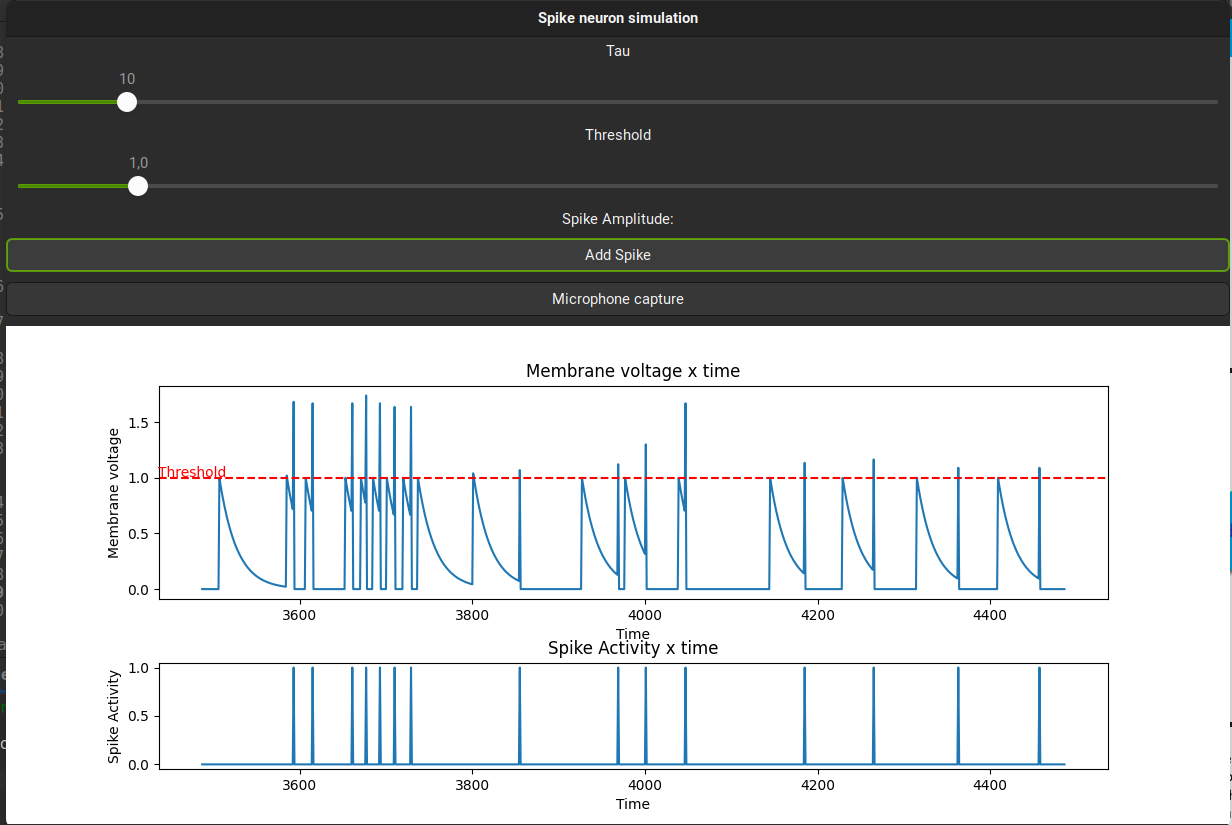
\includegraphics[width=0.6\linewidth]{images/spikeNeuronSimulation}
		\caption[Spiking Neuron Simulator]{A simulation a of spiking neuron}
		\label{fig:spikeneuronsimulation}
	\end{figure}
\end{frame}